\chapter{Impuls}

\section{Definition}
Der Impuls ist eine Grösse aus der klassischen Mechanik die durch das zweite
Newtonsche Axiom formuliert wurde als das Produkt aus Masse und 
Geschwindigkeit.

\[ \boxed{\vec{p}=m \cdot \vec{v}}  \] 
\[ \sum\vec{F}=\vec{F}_{Res} = m \cdot \frac{d\vec{v}}{dt} =
	\frac{d}{dt}(m \cdot \vec{v}) = \frac{d\vec{p}}{dt}  \]

\noindent
Der Impuls ist somit eine vektorielle Grösse und kann somit auch wie die
Kraft und Geschwindigkeit komponentenweise zusammengetragen werden.

\[\begin{pmatrix} 
	p_{x_1} + p_{x_2} + \dots + p_{x_n} \\
	p_{y_1} + p_{y_2} + \dots + p_{y_n} \\
	p_{z_1} + p_{z_2} + \dots + p_{z_n} 
\end{pmatrix}
=
\begin{pmatrix}
	p_x \\
	p_y \\
	p_z
\end{pmatrix}
= \vec{p}  \]

\section{Kraftstoss}
Der Kraftstoss $\vec{J}$ beschreibt eine Impulsänderung welche sich aus einer 
Kraft $\vec{F}$ und deren Einwirkungsdauer $\Delta t$ ergibt. Der Kraftstoss 
ist definiert als das Integral der angewandten Kraft über die Einwirkunsdauer.

\[ \boxed{\vec{J} = \int_{t_1}^{t_2} \left(\sum \vec{F} \right) dt =
	\int_{t_1}^{t_2}\vec{F}_{Res}(t)\cdot dt = \vec{p}_2 - \vec{p}_1} \]

\subsection{Durchschnittliche Kraft}
Mit der vorgerigen Definition des Kraftstosses $\vec{J}$ lässt sich nun die
durchschnittliche Kraft im Zeitintervall $\Delta t = t_2 - t_1$ bestimmen.

\begin{figure}[h!]
	\centering
	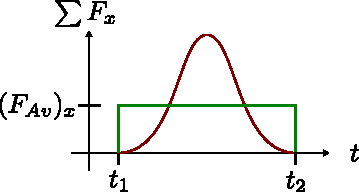
\includegraphics[scale=0.75]{kraftstoss.pdf}
	\caption{Kraftstoss und durchschnittliche Kraft}
	\label{fig:kraftstoss}
\end{figure}

\[ \boxed{\vec{F}_{Av} = \frac{1}{\Delta t} \int_{t_1}^{t_2} \vec{F}(t)dt = 
	\frac{\vec{J}}{\Delta t} = \frac{\vec{p}_2 - \vec{p}_1}{t_2 - t_1}} \]

\section{Impulserhaltung}
In einem abgeschlossenem System\footnote{abgeschlossenes Intertialsystem} 
ist der Gesamtimpuls stets konstant. Der Gesamtimpuls ist die Summe aller 
Impulse in System. Die Impulserhaltung gilt auch ausnahmslos, d.h. auch bei 
Stössen

\[ \vec{p} =
\begin{pmatrix}
	p_{x_1} + p_{x_2} + \dots + p_{x_n} \\
	p_{y_1} + p_{y_2} + \dots + p_{y_n} \\
	p_{z_1} + p_{z_2} + \dots + p_{z_n} 
\end{pmatrix} \]

\section{Stoss}
Mit einem Stoss meint man in der Mechanik eine kurze Wechselwirkung zwischen
verschiedenen Körpern. Hierbei gilt grundsätzlich immer die Impulserhaltung
und je nach Stoss auch die Energieerhaltung.

\subsection{Elastischer Stoss}
Ein elastischer Stoss beschreibt ein Zusammentreffen von Körpern wobei die
Energie erhalten bleibt, d.h. es gitl der Impulserhaltungssatz als auch der
Energieerhatlungssatz. Ein bekanntes Beispiel ist das Kugelstosspendel.

\begin{figure}[h!]
	\centering
	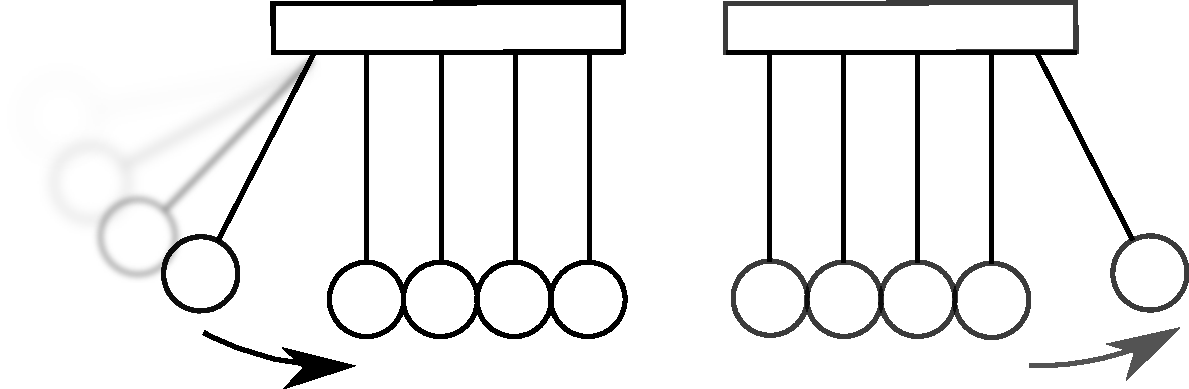
\includegraphics[scale=0.4]{kugelstosspendel.pdf}
	\caption{Kugelstosspendel (Newtons Wiege)}
\end{figure}

\[ \boxed{
	\begin{array}{rcl}
		\vec{p}_{vorher} &= &\vec{p}_{nachher} \\
		E_{kin_{vorher}} &= &E_{kin_{nachher}}
	\end{array}
}\]

\subsection{Inelastischer Stoss}
Ein inelastischer Stoss beschreibt ein Zusammentreffen von Körpern wobei ein
Teil der kinetischen Energie in Verformungsarbeit übergeht. Somit gilt beim
inelastischen Stoss lediglich die Impulserhaltung. 

\[ \boxed{
	\begin{array}{rcl}
		\vec{p}_{vorher} &= &\vec{p}_{nachher} \\
		E_{kin_{vorher}} &\neq &E_{kin_{nachher}}
	\end{array}
} \]

\noindent
Es gibt beim inelastischen Stoss noch den Spezialfall des vollkommen 
inelastischen Stosses. Dies beschreibt ein solches Zusammentreffen, so dass
der maximal mögliche Anteil der kinetischen Energie in innere Energie
umgewandelt wird. Geschieht solch ein Stoss so kleben die Körper zusammen
und bewegen sich mit der selben Geschwindigkeit fort.

\[ \boxed{
	\begin{array}{rcl}
		\vec{p}_{vorher} &= & \vec{p}_{nachher} \\
		\vec{p_1} + \dots + \vec{p}_n &= &\vec{p}_{nachher} \\
		m_1 \cdot \vec{v_1} + \dots + m_n \cdot \vec{p}_n&= 
			& (m_1 + \dots + m_n)\cdot \vec{v}_{nachher}
	\end{array}
} \]

\noindent
Ein gutes Beispiel für solch einen vollkommen inelastischen Stoss ist
das Zusammentreffen von Knetmassen. Diese setzen die kinetische Energie
sehr gut in Verformung um.
